\documentclass[12pt, a4paper]{article}
\usepackage{exercise}
\usepackage{amsmath}
\usepackage{amsfonts}
\usepackage{siunitx}
\usepackage[shortlabels]{enumitem}
\usepackage[margin=2.5cm]{geometry}
\usepackage{graphicx}
\usepackage[justification=centering]{caption}
\usepackage[french]{babel}
\usepackage[upright]{fourier}

\graphicspath{ {./rsc/} }

\sisetup{inter-unit-product=\ensuremath{{}\cdot{}}}
\renewcommand{\ExerciseHeader}
{
  \par\noindent
  \textbf{\large \ExerciseName\ \ExerciseHeaderNB\ExerciseHeaderTitle\ExerciseHeaderOrigin}%
  \par\nopagebreak\medskip
}

\renewcommand{\ExerciseName}{Exercice}

\newenvironment{conditions}
  {\par\vspace{\abovedisplayskip}\noindent\begin{tabular}{>{$}l<{$} @{${\quad}={\quad}$} l}}
  {\end{tabular}\par\vspace{\belowdisplayskip}}

\begin{document}
    \title{Exercices du Chapitre Images et Couleurs \\ \Large{Pages 327-330}}
    \author{Diego Van Overberghe}
    \date{27 Mai 2020}
    \maketitle

    \begin{Exercise}[number={11}]
        \begin{enumerate}[a.]
            \item   $\overline{OA}=-6{,}2$
            \item   $\overline{OA'}=6{,}2$
            \item   $f'=\left(\frac{1}{\overline{OA'}}-\frac{1}{\overline{OA}}\right)^{-1}=3{,}1$
            \item   $\overline{AB}=1{,}5$
            \item   $\overline{A'B'}=-1{,}5$
        \end{enumerate}
    \end{Exercise}

    \begin{Exercise}[number={14}]
        \begin{enumerate}[1.]
            \item   \begin{enumerate}[a.]
                        \item	Position de $\overline{A'B'}=5{,}2$
                        \item   L'image est réele.
                        \item   L'image est à l'envers.
                        \item   Taille de $\overline{A'B'}=1{,}6$
                        \item   $\overline{\gamma}=\frac{\overline{A'B'}}{\overline{AB}}=-1$
                    \end{enumerate}
            \item   \begin{enumerate}[a.]
                        \item	Position de $\overline{A'B'}=-1{,}9$
                        \item   L'image est virtuelle.
                        \item   L'image est à l'endroit.
                        \item   Taille de $\overline{A'B'}=2{,}8$
                        \item   $\overline{\gamma}=\frac{\overline{A'B'}}{\overline{AB}}=1{,}75$
                    \end{enumerate}
        \end{enumerate}
    \end{Exercise}

    \begin{Exercise}[number={19}]
        \begin{enumerate}[1.]
            \item   \begin{enumerate}[a.]
                        \item	Pour obtenir la couleur jaune à partir d'une synthèse additive, il faut des projecteurs rouge et vert.
                        \item   Il faut des projecteurs bleu et rouge.
                    \end{enumerate}	
            \item   Pour obtenir un éclairage blanc à partir des projecteurs rouge vert et bleu, il activer chaqun à 100\%.
            \item   Il est possible de reproduire toutes les couleurs à condition d'avoir des projecteurs avec une luminosité controlable.
            \item   Le modèle de synthèse mis en œuvre est la synthèse additive.
        \end{enumerate}
    \end{Exercise}

    \pagebreak

    \begin{Exercise}[number={21}]
        \begin{enumerate}[1.]
            \item	\begin{enumerate}[a.]
                        \item	La couleur de la lumière incidente est blanc.
                        \item   Les couleurs des lumières transmises sont le rouge et le vert. La couleur de la lumière absorbée est le bleu.
                        \item   La couleur de la lumière observée est le jaune.
                    \end{enumerate}
                    \begin{enumerate}[a.]
                        \item	La couleur de la lumière incidente est jaune.
                        \item   La couleur de la lumière transmise est rouge. La couleur de la lumière absorbée est vert.
                        \item   La couleur de la lumière observée est rouge.
                    \end{enumerate}
                    \begin{enumerate}[a.]
                        \item	La couleur de la lumière incidente est cyan.
                        \item   La couleur de la lumière transmise est vert. La couleur de la lumière absorbée est cyan.
                        \item   La couleur de la lumière observée est le vert.
                    \end{enumerate}
            \item   Pour répondre au a. et au c., on utilise la synthèse additive, pour répondre au b., on utilise la synthèse soustractive.
        \end{enumerate}
    \end{Exercise}

    \begin{Exercise}[number={22}]
        \begin{enumerate}[1.]
            \item	Le filtre bleu transmet le bleu, le filtre vert transmet le vert, le filtre jaune transmet le rouge et le vert, le filtre magenta transmet le rouge et le bleu.
            \item   Le filtre vert ne transmet que la lumière verte, cette lumière est aussi transmise par le filtre jaune, donc, la lumière observée à la sortie sera verte. 
            \item   L'ordre des filtres ne change pas la couleur finale, parce que le filtre transmettera toujours les mêmes couleurs, indépendament de sa position.
            \item   En superposant un filtre magenta et un filtre vert, toute les trois couleurs primaires sont diffusés, à la sortie, on ne voit que du noir.
            \item   Les couleurs vert et magneta sont dites ``complémentaires''.
            \item   La couleur complémentaire du bleu est le jaune, donc en superposant ces deux filtres, la toute la lumière sera absorbée.
        \end{enumerate}
    \end{Exercise}

    \begin{Exercise}[number={23}]
        \begin{enumerate}[1.]
            \item	Cet objet absorbe le vert.
            \item \ \\ \parbox{\linewidth}{
                        \centering\vspace{-\baselineskip}
                        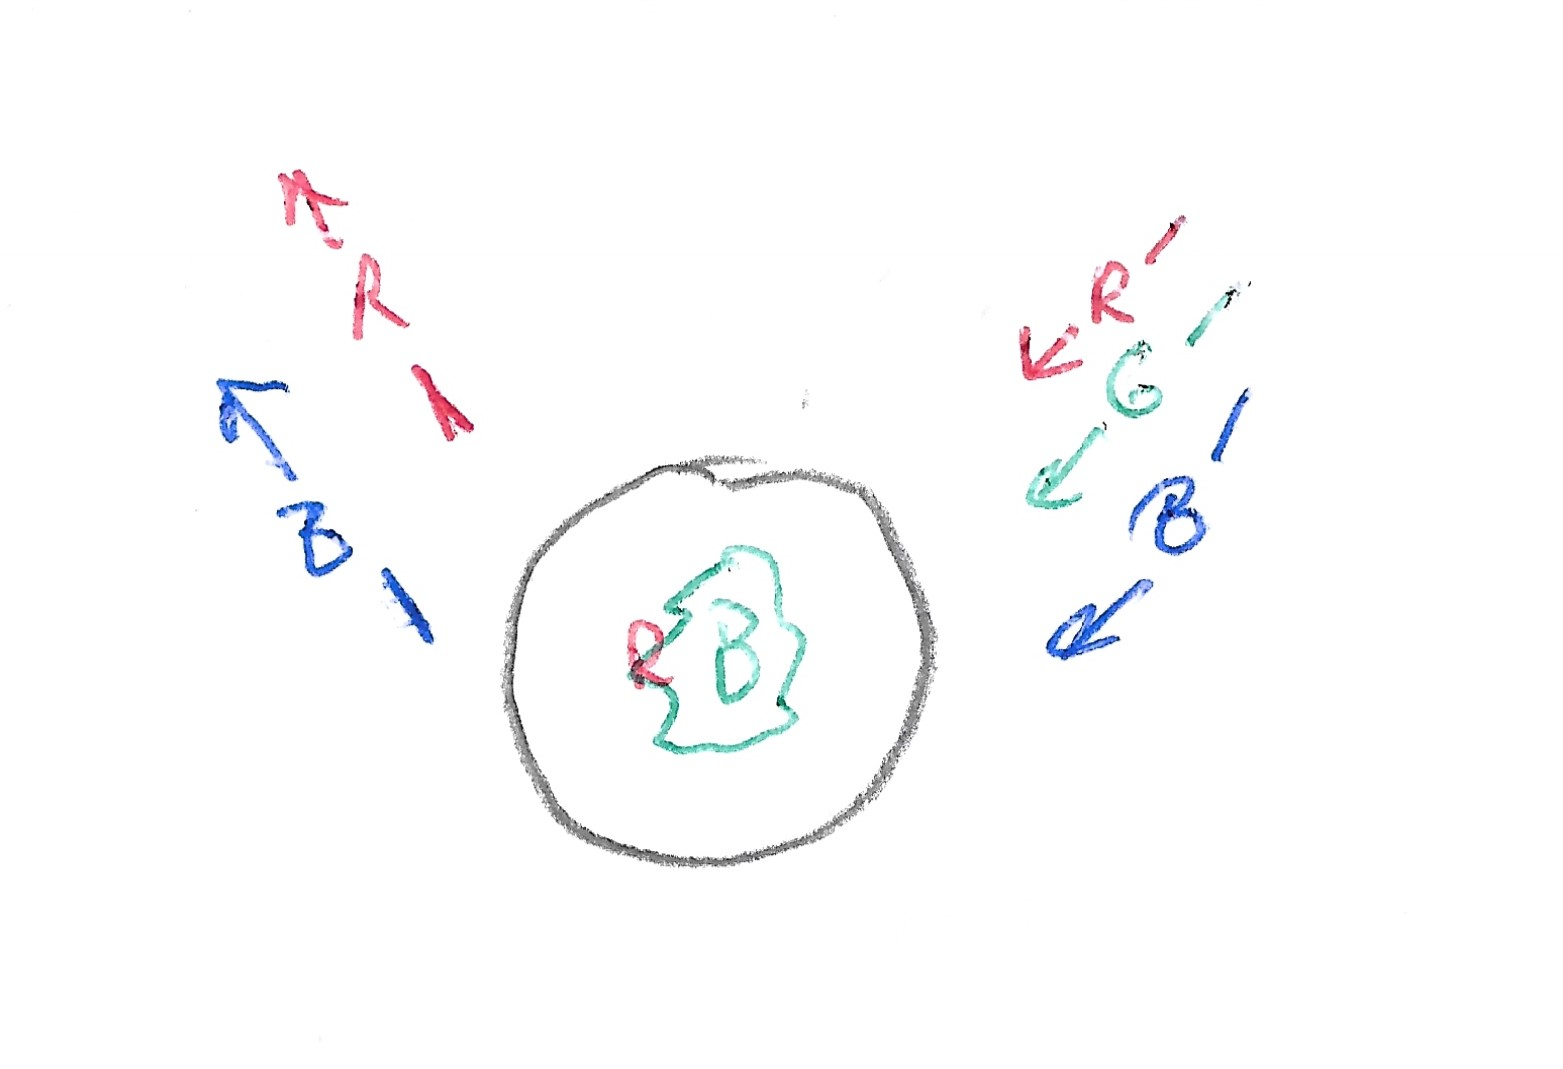
\includegraphics[width=5cm]{EX23img1.jpg}
                        \captionof{figure}{Schema Illustrant les Interactions entre l'Objet et la Lumière}
                    }
            \item   La couleur perçue est le magenta.
        \end{enumerate}
    \end{Exercise}

    \begin{Exercise}[number={24}]
        \begin{enumerate}[1.]
            \item	De gauche à droite: source de la lumière; lumière incidente; lumière transmise; lumière diffusée.
            \item   Les materieaux que rencontrent les rayons de lumière (au niveau de la torche, du filtre et de l'objet).
            \item   Le rouge, le vert et le bleu.
            \item   \begin{enumerate}[a.]
                        \item   La lumière blanche est composée de rouge, vert et bleu. Le filtre transmet la lumière verte et bleue. Le jaune est composé de rouge et vert, donc la lumière diffusée est verte.
                        \item   L'objet est donc perçu comme vert par l'observateur.
                    \end{enumerate}
        \end{enumerate}
    \end{Exercise}

    \begin{Exercise}[number={27}]
        \begin{enumerate}[1.]
            \item	$\large\textcircled{\small{a}}\rightarrow$ Cône bleu; $\large\textcircled{\small{b}}\rightarrow$ Cône vert; $\large\textcircled{\small{c}}\rightarrow$ Cône rouge.
            \item   Parce qu'on possède trois cônes, qui sont adaptés à détecter trois couleurs.
            \item   \begin{enumerate}[a.]
                        \item	La couleur est le bleu foncé.
                        \item   Tous les cônes sont stimulés, cependant, le cône stimulé de manière la plus intense est le cône $\large\textcircled{\small{a}}$, car il a l'intensité relative la plus élevée des trois pour cette longeur d'onde.
                        \item   Bleu foncé.
                    \end{enumerate}
            \item   Lorsque l'œil perçoit la couleur jaune, les récepteurs $\large\textcircled{\small{b}}$ et $\large\textcircled{\small{c}}$ sont stimulés. C'est les récepteurs résponsables de détecter les couleurs vert et rouge, les deux composants du jaune.
        \end{enumerate}
    \end{Exercise}

    \begin{Exercise}[number={29}]
        \begin{enumerate}[1.]
            \item	$\begin{aligned}[t]
                        &\quad \frac{1}{\overline{OA'}}=\frac{1}{\overline{OA}}+\frac{1}{f'} &\\
                        \iff&\quad \overline{OA'}=\left(\frac{1}{-1{,}2\times 10^{2}}+\frac{1}{30}\right)^{-1} &\\
                        \iff&\quad \overline{OA'}=40\ \si{cm}
                    \end{aligned}$
            \item   $\lvert\overline{OA}\rvert>f'\implies$ l'image est réele. \\ Comme l'image est réele, l'image est à l'envers. \\ $\overline{A'B'}=\overline{\gamma}\times\overline{AB}=\frac{\overline{OA'}}{\overline{OA}}\times\overline{AB}=\frac{40}{-1{,}2\times 10^2}\times 2{,}0 \quad \text{soit} \quad \overline{A'B'}=-0{,}67\ \si{cm}$
        \end{enumerate}
    \end{Exercise}

\end{document}